%template voor een afstudeerwerk in LaTeX
\documentclass[dutch,11pt,cite,titlepage]{report}
%''dutch'' voor splitsing en (in emacs) spellingscontrole
\usepackage{babel}   %voor het geval we ook engels nodig hebben
\usepackage{graphicx} %pakket voor includeren figuren
\usepackage{epsfig}
\usepackage[small]{caption}
\usepackage{url}

\usepackage{phd}


% lijst met woorden die LaTeX verkeerd splitst
\hyphenation{vaag-ver-za-me-ling L-vaag-ver-za-me-ling} 

\def\listfigurename{Lijst van figuren}


\begin{document}

\selectlanguage{dutch}


\newcommand{\auteur}{Klaas Bosteels}
\newcommand{\jaar}{2005--2006}
\newcommand{\titel}{Similariteitsgebaseerd rangschikken van afbeeldingen in zoekmachines}
\newcommand{\begeleider}{V. De Witte en S.\ Schulte}
\newcommand{\richting}{licentiaat in de informatica, optie: software-ontwikkeling}

%de volgende lijn kiest de juiste naam van de vakgroepvoorzitter en de promotor
\newcommand{\vakgroep}{Toegepaste Wiskunde en Informatica}
\newcommand{\voorzitter}{prof.\ dr.\ Guido\ Vanden\ Berghe}
\newcommand{\promotor}{prof.\ dr.\ \ E.\ E.\ Kerre}


%het titelblad vergt hier en daar enkele manuele ingrepen i.v.m.
%spatiering en dergelijke
\begin{titlepage}
\renewcommand{\baselinestretch}{1.1}
\Large
\begin{center}
\mbox{}\\[0cm]%de volgende lijnen genereren het tempeltje
\unitlength 1mm

\epsfysize 4cm \epsfclipon\epsffile{ruglogo.eps}\\
%\begin{picture}(0,20)
%\centering
%\put(0,11){\makebox(0,0)[b]{\font\aula=aula34 {\aula a}}}
%\put(0,6){\makebox(0,0)[b]{\font\futura=futura scaled 1100
%                 {\futura UNIVERSITEIT}}}
%\put(0,2){\makebox(0,0)[b]{\font\futura=futura scaled 1100
%                 {\futura GENT}}}
%\put(0,0){\makebox(0,0)[b]{\rule{21mm}{1pt}}}
%\end{picture}\\
{\Large  
Faculteit Wetenschappen\\
Vakgroep \vakgroep\\
Voorzitter: \voorzitter
}\\\vfill
\parbox{14 cm}{
{\Huge\bfseries
\begin{center}
\sf\titel
\end{center}
}
}\\\vfill
door\\ 
{\LARGE \auteur}\\[3.3cm]
%we schrijven ``.\"  i.p.v. ``.'' zodat LaTeX weet dat dit een
%afkorting is (gevolgd door kleine spatie) en niet het einde van een
%zin (gevolgd door lange spatie)
%opmerking: ofwel: prof.\ dr.\ I.\ Lemahieu 
%opmerking: ofwel: prof.\ dr.\ ir.\ W.\ Philips
Promotor: \promotor \\
%Co-promotor: \copromotor \\
Scriptiebegeleiders: \begeleider 
\\\vfill
%        In samenwerking met BARCO GRAPHICS\\
Afstudeerwerk ingediend tot het behalen van de graad van\\
%dit moet uiteraard worden aangepast!
\richting\\[1cm]
Academiejaar \jaar
\end{center}
\renewcommand{\baselinestretch}{1}
\end{titlepage}





%%% Local Variables: 
%%% mode: latex
%%% TeX-master: "total"
%%% End: 
 % de titelpagina
\pagenumbering{roman}
\setcounter{page}{1}
\newpage
\thispagestyle{plain}
\subsection*{Toelating tot bruikleen}
De auteur geeft de toelating dit afstudeerwerk voor consultatie 
beschikbaar te stellen en delen van het afstudeerwerk te copi\"eren voor
persoonlijk gebruik. Elk ander gebruik valt onder de beperkingen van het 
auteursrecht, in het bijzonder met betrekking tot de verplichting de bron 
uitdrukkelijk te vermelden bij het aanhalen van resultaten uit dit 
afstudeerwerk.
\\[2cm]
\auteur\hfill \today
\vfill

\newpage
\thispagestyle{plain}
\subsection*{Dankwoord}
Graag zou ik iedereen willen bedanken die heeft bijgedragen tot de
verwezenlijking van dit eindwerk, in het bijzonder dank ik:
\begin{itemize}
\item mijn caf\'ebaas voor het schenken van het bier;
\item mijn zus, voor het schrijven van mijn thesis;
\item mijn thesisbegeleider \begeleider voor het scheppen van de
  mogelijkheid dit onderzoek te verrichten. 
\end{itemize}
\vfill
%%% Local Variables: 
%%% mode: latex
%%% TeX-master: "total"
%%% End: 
               %het dankwoord.
\newpage
\thispagestyle{plain}

\begin{center}
{\bf \titel }\\[3mm]
door\\
\auteur{} \\
\end{center}
\noindent Afstudeerwerk ingediend tot het behalen van de graad van
\richting
\vspace{3mm}\\
Academiejaar \jaar
\vspace{3mm}\\
\noindent Universiteit Gent\\
Faculteit Wetenschappen\\
\vspace{3mm}\\
\noindent Promotor: \promotor\\
%\noindent Co-promotor: \copromotor\\
\vfill

\noindent {\bf Samenvatting}\\[1mm]
De volgende tekst is een voorbeeld: In ziekenhuizen wordt tegenwoordig
zeer veel digitale data 
gegenereerd. Een groot deel daarvan is afkomstig van medische
beeldvormende modaliteiten zoals Magnetic Resonance Imaging,
Computerized Tomography, Positron Emission Tomography en Single Photon
Emission Computed Tomography. In het Universitair Ziekenhuis van Gent
staan ze in voor meerdere honderden Gbytes aan gegevens per jaar. In
deze thesis wordt nagegaan hoe de data actueel behandeld wordt en wat
de rol van beeldcompressie kan zijn om de opslag- en
transmissieproblemen te verlichten. Wegens de hoge kwaliteitseisen in
de medische sector ligt hierbij de nadruk op verliesloze
compressietechnieken.

Er wordt een vergelijking gemaakt van de performantie van
verschillende algoritmen, waarbij compressieverhouding en
verwerkingssnelheid de belangrijkste parameters zijn. Naast de
state-of-the-art verliesloze beeldcompressietechnieken worden ook
algemene data\-compressietechnieken in de vergelijking betrokken.
Voor MR- en CT-beelden levert de beeldcompressietechniek CALIC de
grootste compressie op, terwijl voor PET- en SPECT-beelden de
datacompressietechnieken STAT en BZIP de beste zijn. Wanneer de
verwer\-kingssnelheid belangrijker is dan de compressieverhouding,
wordt er het best geopteerd voor de datacompressietechnieken GZIP of
COMPRESS.

Verder wordt ook onderzocht hoe driedimensionale predictieve
technieken de redundantie in medische volumebeelden kunnen
uitbuiten. Er wordt aangetoond dat lineaire predictie daar niet in
slaagt. Door middel van context-modellering wordt echter wel een
toename van de compressie bekomen.


\vspace{5mm}

\noindent {\bf Trefwoorden}\\[1mm]
verliesloze beeldcompressie, medische beeldensets

              %samenvatting  van de thesis
\renewcommand{\baselinestretch}{1}

\tableofcontents %genereert de inhoudstafel
%\listoffigures
%\listoftables
%\clearpage

\renewcommand{\baselinestretch}{1}
\pagenumbering{arabic}
\setcounter{page}{1}




\chapter{Inleiding}

Op dit eigenste moment zijn er waarschijnlijk enkele honderden \defin{spiders} actief op internet.
Die computerprogramma's, die soms ook \defin{robots} of \defin{wanderers} worden genoemd, reizen
het internet rond om bepaalde documenten -- in het bijzonder beelden -- te localiseren. Ze indexeren
de gevonden documenten in een databank, die dan doorzocht kan worden door een zoekmachine. 
Zoekmachines zoals \emph{Google} en \emph{Yahoo} hebben op die manier reeds databanken
opgebouwd die meer dan een miljard beelden bevatten. Het wordt bijgevolg steeds belangrijker
om manieren te vinden om die gigantische collecties van beelden op een effici\"ente wijze
te doorzoeken.


\section{Tekstgebaseerd zoeken van beelden}

Alle belangrijke bestaande zoekmachines bieden \defin{text-based image retrieval} (TBIR) aan. 
Figuur~\ref{fig:tbir} toont de algemene architectuur van die machines. Elk beeld 
wordt voorzien van tekstuele annotaties, zoals bijvoorbeeld de 
bestandsnaam of woorden uit de webpagina waarvan het deel uitmaakt. Die annotaties
worden gebruikt voor het indexeren van de beelden in de databank.

De gebruiker van een TBIR-systeem start een zoekactie door \'e\'en of meerdere trefwoorden door te geven
aan het systeem. Het systeem vergelijkt die trefwoorden vervolgens met de annotaties uit
de databank. De beelden waarvan er annotaties overeenkomen met een trefwoord, maken
deel uit van het resultaat van de query. Daarvoor is het uiteraard niet nodig om alle beelden
uit de databank te overlopen, vermits de databank ge\"indexeerd is op de annotaties. 

\section{Inhoudgebaseerd zoeken van beelden}

Figuur~\ref{fig:resultaten_orig_banaan} toont de eerste 25 zoekresultaten die teruggegeven 
worden door \emph{Yahoo Image Search} voor de query ``banaan''. Uit dat voorbeeld
blijkt dat de tekstgebaseerde aanpak in de praktijk niet altijd even goed werkt. Men is 
daarom op zoek gegaan 
naar manieren om het zoeken te baseren op de visuele inhoud van de beelden 
\cite{smeulders:cbir_end_of_early_years}. Zo zijn de \defin{content-based image retrieval} (CBIR) systemen 
\cite{veltcamp:cbirs} ontstaan. 
De algemene architectuur van een dergelijk systeem wordt ge\"illustreerd door
figuur~\ref{fig:cbir}. Er wordt gebruik gemaakt van een proces dat \defin{kenmerkextractie}
(\definas{feature extraction}{(visual) feature extraction}) genoemd wordt \cite{rui:image_retr}. Dat proces zet een beeld om in een 
\defin{kenmerkvector} (\defin{feature vector}). Met behulp van multidimensionale indexering kan die
vector dan gebruikt worden als alternatief voor de tekstuele annotaties bij TBIR.

\begin{figure}[bp]
\vspace{10pt}
\centering
\begin{tabular}{@{}ccccc@{}}
\includegraphics[scale=0.6]{images/banaan_orig_1_1.eps} &
\includegraphics[scale=0.5]{images/banaan_orig_1_2.eps} &
\includegraphics[scale=0.6]{images/banaan_orig_1_3.eps} &
\includegraphics[scale=0.4]{images/banaan_orig_1_4.eps} &
\includegraphics[scale=0.5]{images/banaan_orig_1_5.eps}\vspace{10pt}\\
\includegraphics[scale=0.6]{images/banaan_orig_2_1.eps} &
\includegraphics[scale=0.7]{images/banaan_orig_2_2.eps} &
\includegraphics[scale=0.6]{images/banaan_orig_2_3.eps} &
\includegraphics[scale=0.6]{images/banaan_orig_2_4.eps} &
\includegraphics[scale=0.6]{images/banaan_orig_2_5.eps}\vspace{10pt}\\
\includegraphics[scale=0.6]{images/banaan_orig_3_1.eps} &
\includegraphics[scale=0.6]{images/banaan_orig_3_2.eps} &
\includegraphics[scale=0.6]{images/banaan_orig_3_3.eps} &
\includegraphics[scale=0.6]{images/banaan_orig_3_4.eps} &
\includegraphics[scale=0.6]{images/banaan_orig_3_5.eps}\vspace{10pt}\\
\includegraphics[scale=0.6]{images/banaan_orig_4_1.eps} &
\includegraphics[scale=0.8]{images/banaan_orig_4_2.eps} &
\includegraphics[scale=0.6]{images/banaan_orig_4_3.eps} &
\includegraphics[scale=0.6]{images/banaan_orig_4_4.eps} &
\includegraphics[scale=0.6]{images/banaan_orig_4_5.eps}\vspace{10pt}\\
\includegraphics[scale=0.6]{images/banaan_orig_5_1.eps} &
\includegraphics[scale=0.6]{images/banaan_orig_5_2.eps} &
\includegraphics[scale=0.6]{images/banaan_orig_5_3.eps} &
\includegraphics[scale=0.6]{images/banaan_orig_5_4.eps} &
\includegraphics[scale=0.6]{images/banaan_orig_5_5.eps}
\end{tabular}
\vspace{10pt}
\caption{\label{fig:resultaten_orig_banaan}De eerste 25 zoekresultaten voor de query "banaan".}
\end{figure}

De meeste CBIR-systemen werken volgens het \defin{query-by-example} principe. Dat houdt in dat de
gebruiker een beeld als voorbeeld opgeeft, waarna het systeem op zoek gaat naar beelden
die visuele gelijkenissen vertonen met dat voorbeeld. Daartoe wordt eerst de kenmerkvector van
het opgegeven beeld bepaald, om die vervolgens te vergelijken met de kenmerkvectoren in
de databank. Het uiteindelijke resultaat bestaat uit de beelden uit de databank 
waarvan de overeenkomstige vectoren grote similariteit vertonen met de vector van het 
voorbeeld. 
%Doordat de databank ge\"indexeerd is op de kenmerkvectoren, is het niet nodig
%om alle vectoren te overlopen.

\begin{figure}[!b]
\vspace{10pt}
\centering
\subfigure[]{
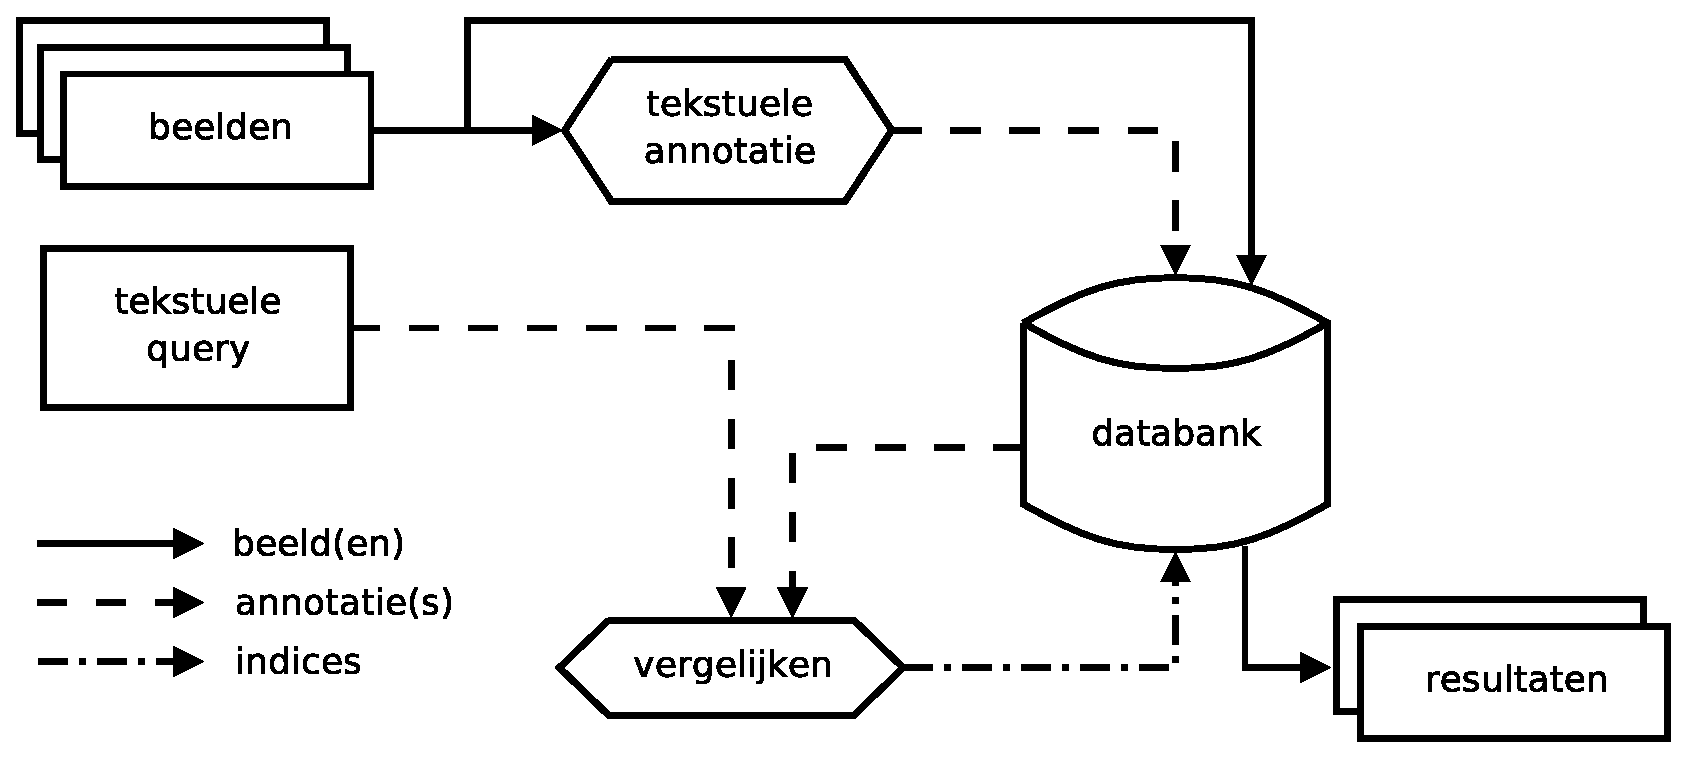
\includegraphics[width=9cm]{images/tbir.eps}
\label{fig:tbir}
}
\vspace{5pt}
\subfigure[]{
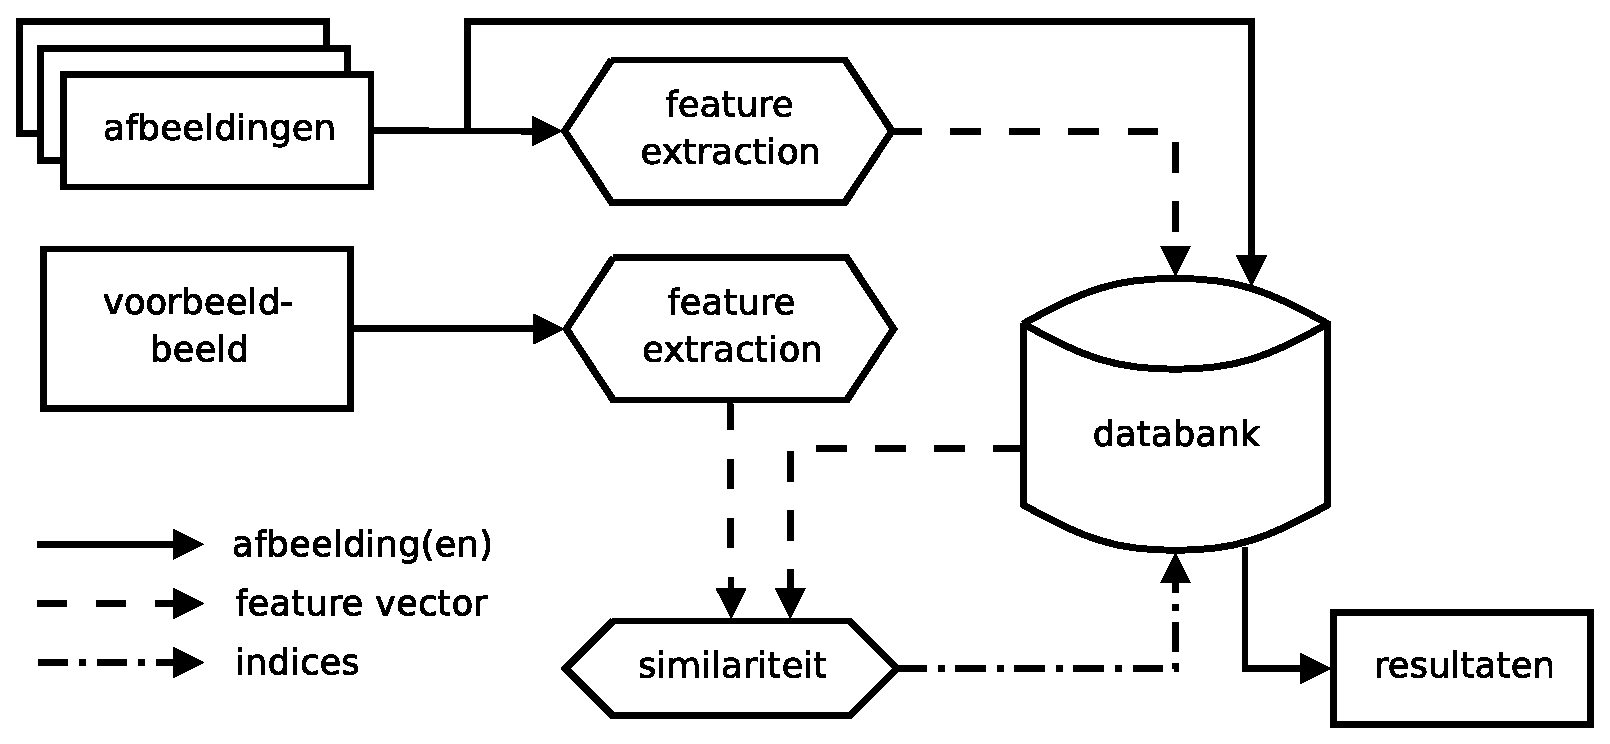
\includegraphics[width=9cm]{images/cbir.eps}
\label{fig:cbir}
}
\vspace{5pt}
\subfigure[]{
\includegraphics[width=9cm]{images/simgeb_rangschikken.eps}
\label{fig:simgeb_rangschikken}
}
\caption{\label{fig:cbir_en_tbir}Algemene architectuur van (a) een TBIR-systeem, 
(b) een CBIR-systeem en (c) een systeem dat het similariteitsgebaseerd rangschikking
van de zoekresultaten implementeert.}
\end{figure}

\section{Similariteitsgebaseerd rangschikken van de zoekresultaten}

Doordat CBIR-systemen zeer complex zijn, is het op dit moment nog niet mogelijk om ze te gebruiken voor het 
doorzoeken van zeer omvangrijke databanken. Bovendien beschikt de gebruiker niet altijd over
een geschikt voorbeeld. Dat probleem kan eventueel nog opgelost worden door gebruik
te maken van een voorbeeld-schets, maar ook dat is in de praktijk niet altijd even handig.
Het is bijgevolg zinvol om te zoeken naar manieren om inhoudgebaseerde aspecten toe te voegen aan
TBIR-systemen. 

De manier die we in deze scriptie bespreken, is het 
similariteitsgebaseerd rangschikken van de zoekresultaten van een TBIR-systeem. 
Figuur~\ref{fig:simgeb_rangschikken} toont de algemene architectuur van een systeem
dat die techniek implementeert. We verwachten
nog steeds dat de gebruiker een tekstuele query opgeeft, waarop het systeem antwoordt met een 
lijst van beelden die overeenkomen met die query. Daarna heeft de gebruiker echter ook nog 
de mogelijkheid om een verzameling van voorbeelden te kiezen uit die lijst. Het 
systeem zorgt er vervolgens voor dat de zoekresultaten gerangschikt worden in 
volgorde van similariteit met de voorbeelden.

Beschouw bijvoorbeeld de zoekresultaten uit figuur~\ref{fig:resultaten_orig_banaan}. Als
we effectief op zoek zijn naar een beeld van een banaan, dan zijn het
eerste en het voorlaatste beeld vrij goede resultaten. Bij een uitbreiding die het 
similariteitsgebaseerd rangschikken implementeert, kunnen die beelden als
voobeeld opgegeven worden. Via \'e\'en van de technieken die we verder in dit
eindwerk bespreken, bekomen we dan de rangschikking uit 
figuur~\ref{fig:resultaten_sorted_banaan}. Die rangschikking kan eventueel nog 
verder verfijnd worden door bijkomende voorbeelden op te geven.

\begin{figure}[!bp]
\vspace{10pt}
\centering
\begin{tabular}{@{}ccccc@{}}
\includegraphics[scale=0.6]{images/banaan_sorted_1_1.eps} &
\includegraphics[scale=0.6]{images/banaan_sorted_1_2.eps} &
\includegraphics[scale=0.6]{images/banaan_sorted_1_3.eps} &
\includegraphics[scale=0.6]{images/banaan_sorted_1_4.eps} &
\includegraphics[scale=0.6]{images/banaan_sorted_1_5.eps}\vspace{10pt}\\
\includegraphics[scale=0.6]{images/banaan_sorted_2_1.eps} &
\includegraphics[scale=0.6]{images/banaan_sorted_2_2.eps} &
\includegraphics[scale=0.6]{images/banaan_sorted_2_3.eps} &
\includegraphics[scale=0.6]{images/banaan_sorted_2_4.eps} &
\includegraphics[scale=0.6]{images/banaan_sorted_2_5.eps}\vspace{10pt}\\
\includegraphics[scale=0.6]{images/banaan_sorted_3_1.eps} &
\includegraphics[scale=0.6]{images/banaan_sorted_3_2.eps} &
\includegraphics[scale=0.6]{images/banaan_sorted_3_3.eps} &
\includegraphics[scale=0.6]{images/banaan_sorted_3_4.eps} &
\includegraphics[scale=0.6]{images/banaan_sorted_3_5.eps}\vspace{10pt}\\
\includegraphics[scale=0.6]{images/banaan_sorted_4_1.eps} &
\includegraphics[scale=0.6]{images/banaan_sorted_4_2.eps} &
\includegraphics[scale=0.6]{images/banaan_sorted_4_3.eps} &
\includegraphics[scale=0.6]{images/banaan_sorted_4_4.eps} &
\includegraphics[scale=0.6]{images/banaan_sorted_4_5.eps}\vspace{10pt}\\
\includegraphics[scale=0.6]{images/banaan_sorted_5_1.eps} &
\includegraphics[scale=0.6]{images/banaan_sorted_5_2.eps} &
\includegraphics[scale=0.6]{images/banaan_sorted_5_3.eps} &
\includegraphics[scale=0.8]{images/banaan_sorted_5_4.eps} &
\includegraphics[scale=0.6]{images/banaan_sorted_5_5.eps}
\end{tabular}
\vspace{10pt}
\caption{\label{fig:resultaten_sorted_banaan}De eerste 25 gerangschikte zoekresultaten voor de query "banaan".}
\end{figure}

\chapter{Wiskundige fundamenten}

In dit hoofdstuk introduceren we eerst enkele basisbegrippen uit de vaagverzamelingenleer. 
Daarna geven we een overzicht van de similariteitsmaten en aggregatieoperatoren waarvan
we in het vervolg van deze scriptie gebruik zullen maken.

\section{Vaagverzamelingen}

De collectie van alle mogelijke elementen noemen we het \emph{universum} (bijvoorbeeld de
natuurlijke getallen). Een verzameling bevat bepaalde elementen uit dit universum (bijvoorbeeld de 
verzameling van de priemgetallen). 

In het geval van een \emph{scherpe verzameling}, behoort elk 
element uit het universum wel of niet tot de verzameling. Andere mogelijkheden zijn er
niet. Een dergelijke verzameling kan bijgevolg 
gerepresenteerd worden door een \emph{karakteristieke afbeelding}, die elk element uit het 
universum afbeeldt op 0 of 1. Dit getal noemen we de \emph{lidmaatschapsgraad} van het element 
in kwestie. De klasse van scherpe verzamelingen in een universum $X$ stellen we voor door 
$\mathcal{P}(X)$.
\begin{definitie}
Zij $X$ een universum. De karakteristieke afbeelding $\mu_A$ van een scherpe verzameling $A$ in $X$
wordt gedefinieerd als de $X - \{0,1\}$ afbeelding:
$$
\begin{array}{lllll}
\mu_A: 	& X & \to 		& \{0,1\}	& \\
		& x & \mapsto 	& 1,		& \textrm{ als } x \in A \\
		& x & \mapsto 	& 0,		& \textrm{ als } x \notin A
\end{array}
$$
\end{definitie}

Bij een \emph{vaagverzameling} kunnen alle waarden tussen 0 en 1 als lidmaatschapsgraad 
voorkomen. De karakteristiek afbeelding is in dit geval dus een $X - [0,1]$ afbeelding:
\begin{definitie}
Zij $X$ een universum. Een vaagverzameling $A$ in $X$ wordt gekarakteriseerd door een $X - [0,1]$
afbeelding  $\mu_A$:
$$
\begin{array}{lllll}
\mu_A: 	& X & \to 		& [0,1]	& \\
		& x & \mapsto 	& \mu_A(x),		& \forall x \in A
\end{array}
$$
\end{definitie}
\noindent
Een element $x \in X$ behoort dus tot de vaagverzameling $A$ met lidmaatschapsgraad $\mu_A(x)$.
Voor de eenvoud zullen we in het vervolg $\mu_A(x)$ steeds noteren als $A(x)$. We zullen dus 
met andere woorden geen onderscheid meer maken tussen de vaagverzameling en de 
lidmaatschapsfunctie. Voor de klasse van vaagverzamelingen in een universum $X$ gebruiken we
de notatie $\mathcal{F}(X)$.

De \emph{drager} en de \emph{kern} van een vaagverzameling zijn twee belangrijke begrippen: 
\begin{definitie}
De drager van een vaagverzameling $A$ in $X$ wordt gedefinieerd als:
$$
supp\ A = \{x \in X \mid A(x) > 0\} 
$$
\end{definitie}
\begin{definitie}
De kern van een vaagverzameling $A$ in $X$ defini\"eren we als volgt:
$$
ker\ A = \{x \in X \mid A(x) = 1\}
$$
\end{definitie}
\noindent
Ook het begrip \emph{cardinaliteit} speelt vaak een belangrijke rol. De cardinaliteit van een 
een eindige scherpe verzameling wordt gegeven door het aantal elementen in die verzameling. 
Dit concept kan uitgebreid worden naar vaagverzamelingen door gebruik te maken van het begrip 
\emph{sigma count}:
\begin{definitie}
De sigma count van een vaagverzameling $A$ met eindige drager in een universum $X$ wordt
gedefinieerd door:
$$
|A|=\sum_{x \in X} A(x)
$$
\end{definitie}

\section{Bewerkingen op vaagverzamelingen}

We beginnen met het defini\"eren van de begrippen \emph{negator}, \emph{conjunctor} en 
\emph{disjunctor}. Deze operatoren zijn uitbreidingen van de klassieke logische operatoren
$\lnot$ (negatie), $\land$ (conjunctie) en $\lor$ (disjunctie).
\begin{definitie}
Een negator $\mathcal{N}$ op $[0,1]$ is een dalende $[0,1] - [0,1]$ afbeelding die voldoet
aan de randvoorwaarden $\mathcal{N}(0)=1$ en $\mathcal{N}(1)=0$. 
\end{definitie}
\begin{definitie}
Een conjunctor $\mathcal{C}$ op $[0,1]$ is een stijgende $[0,1]^2 - [0,1]$ afbeelding die voldoet aan de
randvoorwaarden $\mathcal{C}(0,0)=\mathcal{C}(0,1)=\mathcal{C}(1,0)=0$ en $\mathcal{C}(1,1)=1$.
\end{definitie}
\begin{definitie}
Een disjunctor $\mathcal{D}$ op $[0,1]$ is een stijgende $[0,1]^2 - [0,1]$ afbeelding die voldoet
aan de randvoorwaarden $\mathcal{D}(1,0)=\mathcal{D}(0,1)=\mathcal{D}(1,1)=1$ en 
$\mathcal{D}(0,0)=0$.
\end{definitie}

De meest gebruikte negator is de standaardnegator $N_S$. Het minimum $C_M$ en het algebra\"isch 
product $C_P$ zijn veelgebruikte conjunctors. Bij de disjunctors zijn het maximum $D_M$ en de
probabilistische som $D_P$ dan weer populaire mogelijkheden. Deze operatoren worden als 
volgt gedefinieerd:
$$
\begin{array}{r@{\quad=\quad}l}
N_S(x) & 1 - x \\
C_M(x,y) & min(x,y) \\
C_P(x,y) & x \cdot y \\
D_M(x,y) & max(x,y) \\
D_P(x,y) & x +y - x \cdot y,
\end{array}
$$
voor alle $(x,y)$ in $[0,1]^2$.

We kunnen de bovenstaande operatoren nu gebruiken om de klassieke verzameltechnische bewerkingen 
$co$ (complement), $\cap$ (doorsnede) en $\cup$ (unie) te
veralgemenen tot bewerkingen op vaagverzamelingen.
\begin{definitie}
Het $\mathcal{N}$-complement $co_\mathcal{N} A$ van een vaagverzameling $A$ in $X$ wordt gedefinieerd
door de volgende vaagverzameling in X:
$$
(co_\mathcal{N} A)(x) = \mathcal{N}(A(x)),
$$
voor alle $x$ in $X$, met $\mathcal{N}$ een negator.
\end{definitie}
\begin{definitie}
De $\mathcal{C}$-doorsnede $A \cap_\mathcal{C} B$ van twee vaagverzamelingen $A$ en $B$ in $X$
wordt gedefinieerd door de volgende vaagverzameling in $X$:
$$
(A \cap_\mathcal{C} B)(x) = \mathcal{C}(A(x),B(x)),
$$
voor alle $x$ in $X$, met $\mathcal{C}$ een conjunctor.
\end{definitie}
\begin{definitie}
De $\mathcal{D}$-unie $A \cup_\mathcal{D} B$ van twee vaagverzamelingen $A$ en $B$ in $X$ wordt gedefinieerd door de
volgende vaagverzameling in $X$:
$$
(A \cup_\mathcal{D} B)(x) = \mathcal{D}(A(x),B(x)),
$$
voor alle $x$ in $X$, met $\mathcal{D}$ een disjunctor.
\end{definitie}

In het vervolg van deze scriptie zullen we doorgaands 
$(\mathcal{N},\mathcal{C},\mathcal{D})=(N_S,C_M,D_M)$ kiezen. We voeren daarom de volgende
verkorte notaties in:
$$
\begin{array}{r@{\quad=\quad}l}
A^c 		& co_{N_S} A \\
A \cap B 	& A \cap_{C_M} B \\
A \cup B	& A \cup_{D_M} B,
\end{array}
$$
waarbij $A$ en $B$ vaagverzamelingen zijn.


\section{L-vaagverzamelingen}

\section{Aggregatieoperatoren} 


\chapter{Similariteit}

\section{Pixel-gebaseerd}
\section{Kleur-gebaseerd}

\chapter{Aggregatie}

\section{Aggregatie van similariteiten}
\section{Aggregatie van afbeeldingen}


\chapter{Implementatie}

\section{Imilarity}
\section{Giggle}


\nocite{*}
%\selectlanguage{english} % vermits de meeste referenties in het engels zijn.
\bibliographystyle{alpha} 

\bibliography{thesis}           % dit bestand bevat informatie die
                                %door bibtex wordt gelezen

\end{document}